
Modules allow programmers to define an API for code in the large. The code might consist of multiple classes, multiple files, several functions, and various auxiliary utilities including templates. By using the keyword export, you can specify what is exported as the API of a module that wraps all code that provides a certain functionality. Thus, we can define a clean API of a component implemented in various files.

Let us look at a few simple examples that declare a module in one file and then use this module in another file.

\mySubsubsection{16.1.1}{Implementing and Exporting a Module}

The specification of the API of a module is defined in its primary interface (the official name is primary module interface unit), which each module has exactly once:

\filename{modules/mod0.cppm}

\begin{cpp}
export module Square; // declare module Square

int square(int i);

export class Square {
private:
	int value;
public:
	Square(int i)
	: value{square(i)} {
	}
	int getValue() const {
		return value;
	}
};
	
export template<typename T>
Square toSquare(const T& x) {
	return Square{x};
}
	
int square(int i) {
	return i * i;
}
\end{cpp}

The first thing you might recognize is that the file uses a new file extension: .cppm. The file extension of module files is not clear yet. We will discuss the handling of module files by compilers later.

The key entry for the primary interface is the line that declares and exports the module using the name Square:

\begin{cpp}
export module Square; // declare module Square
\end{cpp}

Note that the name is used only as an identifier to import the module. It does not introduce a new scope or namespace. Any name exported by the module is still in the scope it was in when it was exported.

The name of a module may contain periods, While periods are not valid in any other kinds of identifiers used in C++, a period as a character of a module name identifier is valid and has no special meaning. For example:

\begin{cpp}
export module Math.Square; // declare module “Math.Square”
\end{cpp}

This has no other effect than naming the module with “MathDotSquare,” except that using a period has a visual effect. Periods can be used to signal some logical relationships between modules established by a component or project. Using them has no syntactic or formal consequences.

The public API of a module is defined by everything that is explicitly exported using the keyword export. In this case, we export the class Square and the function template toSquare<>():

\begin{cpp}
export class Square {
	...
};

export template<typename T>
Square toSquare(const T& x) {
	...
}
\end{cpp}

Everything else is not exported and cannot be used directly by code that imports the module (we will discuss later how non-exported module symbols may be reachable but not visible). Therefore, the function square() declared without export cannot be used by code that imports this module.

The file looks like a header file with the following differences:

\begin{itemize}
\item 
We have the line with the module declaration.

\item 
We have symbols, types, functions (even templates) that are exported with export.

\item 
We do not need inline to define functions.

\item 
We do not need preprocessor guards.
\end{itemize}

However, the module file is not just an improved header file. A module file can play the role of both a header and a source file. It can contain declarations and definitions. Furthermore, in a module file, you do not have to specify a definition with inline or within preprocessor guards. Entities exported by modules cannot violate the One Definition Rule when imported by different translation units.

Each module must have exactly one primary interface file with its specified name. As you can see, the name of the module does not conflict with any symbol within the module. It also does not implicitly introduce a namespace. Therefore, a module can have the name of its (major) namespace, class, or function. In practice, module names may often fit with the namespace of the symbols exported. This, however, is something you have to implement explicitly.

\mySubsubsection{16.1.2}{Compiling Module Units}

As you can see, a module file may have both declarations and definitions. In the traditional sense, it can be seen as a combination of header and source file. The consequence is that you have to do two things with it:

\begin{itemize}
\item 
\textbf{Precompile the declarations} (including all generic code), which converts the declarations into a compilerspecific format

\item 
\textbf{Compile the definition}, which creates the usual object files
\end{itemize}

\begin{center}
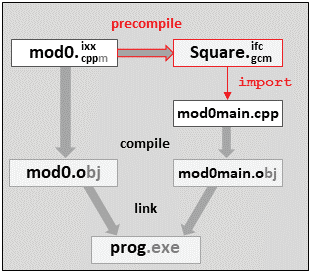
\includegraphics[width=0.6\textwidth]{content/chapter16/images/1.png}\\
Figure 16.1. Dealing with C++ modules
\end{center}

Given that we have the primary module interface mod0.cppm above, we have to deal with it in two ways as Figure 16.1 demonstrates:

\begin{itemize}
\item 
We have to precompile mod0.cppm to create a precompiled module file that contains all exported declarations including precompiled template definitions. It is identified by the name of the module Square, not by the name of the source file.

\item
We have to compile mod0.cppm to create an object file mod0.o or mod0.obj with the assembler code of all definitions that can be compiled directly.
\end{itemize}

As already stated, there are no specific file extensions required for source module files. I use .cppm here. There is also no standardized suffix for precompiled module files. It is up to the compiler to decide about them. By default, we currently have the following situation:

\begin{itemize}
\item 
gcc/g++ uses .gcm for precompiled files (and places them in a subdirectory gcm.cache).

\item
Visual C++ uses .ifc for precompiled files (and places them in the local directory).
\end{itemize}

We will discuss file suffixes and options for dealing with module units later in detail.

Note that a successful compilation of a source file that imports modules requires that the precompiled artifact of the module is available. Thus, you have to precompile mod0.cppm before you can compile mod0test.cpp. If you do not follow the correct order, you might import a version of the specified module that is not up to date. As a consequence, cyclic import dependencies are not allowed.

In contrast to other programming languages, C++ does not require a module to have a special file name or be in a special directory. Any C++ file can define a module (but only one) and the name of the module need not have anything to do with the name or location of the file.

Of course, it makes good sense to keep file names and module names synchronized somehow. However, that decision ultimately depends on your preferences and the constraints of the configuration management and build systems that you use.

\mySubsubsection{16.1.3}{Importing and Using a Module}

To use the code of a module in a program, you have to import the module under its name. Here is a simple example of a program using just the module Square defined above:

\filename{modules/mod0main.cpp}

\begin{cpp}
#include <iostream>

import Square; // import module “Square”

int main()
{
	Square x = toSquare(42);
	std::cout << x.getValue() << '\n';
}
\end{cpp}

With

\begin{cpp}
import Square; // import module “Square”
\end{cpp}

we import all exported symbols from the module Square. This means that we can then use the exported class Square and the function template toSquare<>().

Using any symbol from the module that is not exported results in a compile-time error:

\begin{cpp}
import Square; // import module ”Square”

square(42) // ERROR: square() not exported
\end{cpp}

Again, note that a module does not automatically introduce a new namespace. We use the exported symbols of the module in the scope they were in when they were exported. If you want to have everything exported from the module in its own namespace, you can exporting the namespace as a whole.

\mySubsubsection{16.1.4}{Reachable versus Visible}

When using modules, a new distinction comes into play: reachability versus visibility. When exporting data, we might not be able to see and directly use a name or symbol of the module; although we might be able to use it indirectly.

Symbols that are reachable but not visible can occur when an exported API provides access to a type that is not exported. Consider the following example:

\begin{cpp}
export module ModReach; // declare module ModReach

struct Data { // declare a type not exported
	int value;
};

export struct Customer { // declare an exported type
private:
	Data data;
public:
	Customer(int i)
	: data{i} {
	}
	Data getData() const { // yield a type not exported
		return data;
	}
};
\end{cpp}

When importing this module, type Data is not visible and therefore cannot be used directly:

\begin{cpp}
import ModReach;
...

Data d{11}; // ERROR: type Data not exported
Customer c{42};
const Data& dr = c.getData(); // ERROR: type Data not exported
\end{cpp}

However, type Data is reachable and that thus be used indirectly:

\begin{cpp}
import ModReach;
...

Customer c{42};
const auto& dr = c.getData(); // OK: type Data is used
auto d = c.getData(); // OK: d has type Data
std::cout << d.value << '\n'; // OK: type Data is used
\end{cpp}

You can even declare an object of type Data as follows:

\begin{cpp}
decltype(std::declval<Customer>().getData()) d; // d has non-exported type Data
\end{cpp}

By using std::declval<>(), we call getData() for an assumed object of type Customer. Therefore, we declare d with the type Data, the return type of getData(), if called for an object of type Customer.

Private module fragments can be used to restrict the reachability of indirectly exported classes and functions.

The visibility and reachability of exported symbols are discussed later in detail.

\mySubsubsection{16.1.5}{Modules and Namespaces}

As already mentioned, symbols of a module are imported in the same scope as when they were exported. In contrast to some other programming languages, C++ modules do not automatically introduce a namespace for a module.

You might therefore use the convention of exporting everything in a module in a namespace with its name. You can do that in two ways:

\begin{itemize}
\item 
Specify the component(s) you want to export with export within the namespace:
 
\begin{cpp}
export module Square; // declare module ”Square”

namespace Square {
	int square(int i);
	
	export class Square {
		...
	};
	
	export template<typename T>
	Square toSquare(const T& x) {
		...
	}
	
	int square(int i) { // not exported
		...
	}
}
\end{cpp}

\item 
Specify everything you want to export in a namespace declared with export:

\begin{cpp}
export module Square; // declare module ”Square”

int square(int i);

export namespace Square {
	class Square {
		...
	};
	
	template<typename T>
	Square toSquare(const T& x) {
		...
	}
}

int square(int i) { // not exported
	...
}
\end{cpp}

\end{itemize}

In both cases, the module exports class Square::Square and Square::toSquare<>() (therefore, the namespace of the symbols is exported, even if not marked with export).

Using the module would now look as follows:

\begin{cpp}
#include <iostream>

import Square; // import module ”Square”

int main()
{
	Square::Square x = Square::toSquare(42);
	std::cout << v.getValue() << '\n';
}
\end{cpp}

